% !TEX encoding = UTF-8 Unicode
%!TEX TS-program = xelatex

\documentclass[12pt]{extarticle}
% extarticle is like article but can handle 8pt, 9pt, 10pt, 11pt, 12pt, 14pt, 17pt, and 20pt text

\def \ititle {Origins of Mind}
 
\def \isubtitle {Lecture 08}
 
\def \iauthor {Stephen A. Butterfill}
\def \iemail{s.butterfill@warwick.ac.uk}
\date{}

%for strikethrough
\usepackage[normalem]{ulem}

\usepackage{pdfpages}


\input{$HOME/Documents/submissions/preamble_steve_handout}

%logic symbol \leftmodels
\usepackage{MnSymbol}

%\bibpunct{}{}{,}{s}{}{,}  %use superscript TICS style bib
%remove hanging indent for TICS style bib
%TODO doesnt work
\setlength{\bibhang}{0em}
%\setlength{\bibsep}{0.5em}


%itemize bullet should be dash
\renewcommand{\labelitemi}{$-$}

\begin{document}

%\raggedcolumns

\begin{multicols*}{3}

\setlength\footnotesep{1em}


\bibliographystyle{newapa} %apalike

%\maketitle
%\tableofcontents




%--------------- 
%--- start paste
\def \ititle {Logic (PH133)}
 
\def \isubtitle {Lecture 3}
 
\begin{center}
 
{\Large
 
\textbf{\ititle}: \isubtitle
 
}
 
 
 
\iemail %
 
\end{center}
 
Readings refer to sections of the course textbook, \emph{Language, Proof and Logic}.
 
 
 
\section{∧Intro and ∨Intro: Compare and Contrast}
 
\emph{Reading:} §6.1
 
\begin{center}
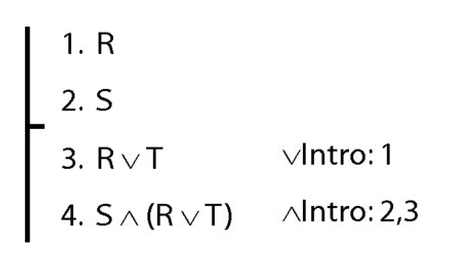
\includegraphics[scale=0.3]{img/proof_unit_212}
\end{center}
\begin{minipage}{\columnwidth}
 
Let us define a new connective with this truth table:
 
\begin{center}
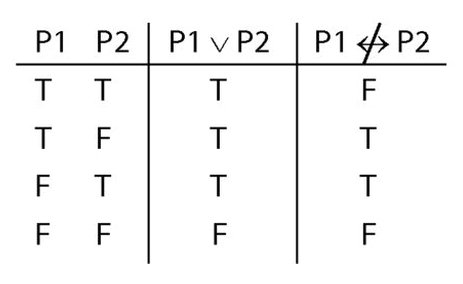
\includegraphics[scale=0.3]{img/tt_not_equivalent.png}
\end{center}
\end{minipage}
 
\begin{minipage}{\columnwidth}
 
The following rule is unacceptable. Why?
 
\begin{center}
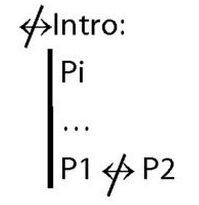
\includegraphics[scale=0.3]{img/rule_not_equivalent_intro_wrong.png}
\end{center}
\end{minipage}
 
 
 
\section{How to Write Proofs}
 
\begin{center}
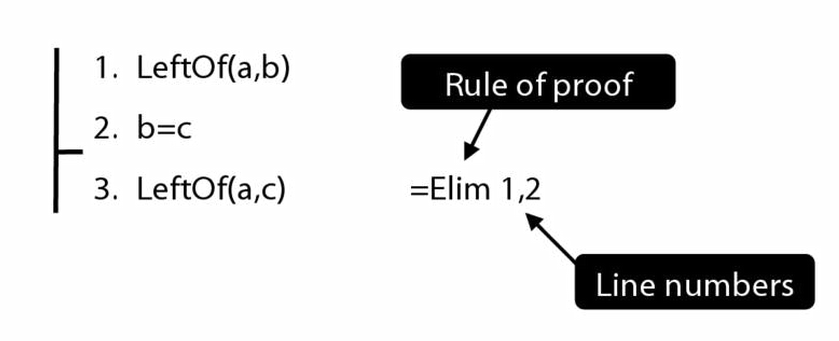
\includegraphics[scale=0.3]{img/how_to_write_proofs.png}
\end{center}
 
 
\section{Rules of Proof for Identity}
 
\emph{Reading:} §2.2
 
\begin{center}
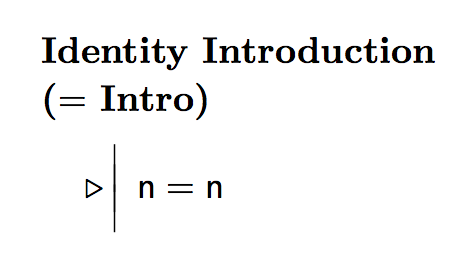
\includegraphics[scale=0.3]{img/rule_identity_intro.png}
\end{center}
\begin{center}
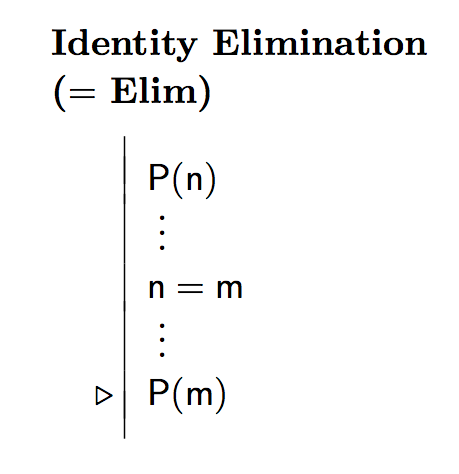
\includegraphics[scale=0.3]{img/rule_identity_elim.png}
\end{center}
\begin{center}
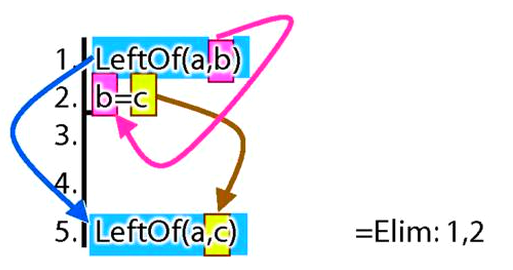
\includegraphics[scale=0.3]{img/proof_identity_example.png}
\end{center}
 
 
\section{Logic Makes Me Die Inside}
 
\emph{Reading:} §2.1
 
 
 
\section{¬, $\bot$}
 
\emph{Reading:} §6.3
 
\begin{center}
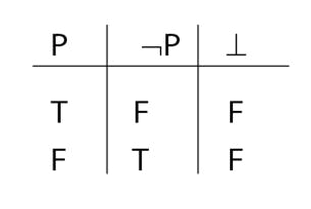
\includegraphics[scale=0.3]{img/tt_contradiction.png}
\end{center}
\begin{center}
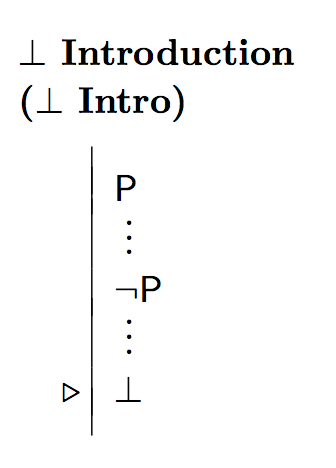
\includegraphics[scale=0.3]{img/rule_contradiction_intro.png}
\end{center}
\begin{center}
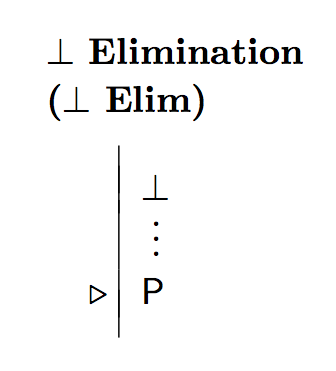
\includegraphics[scale=0.3]{img/rule_contradiction_elim.png}
\end{center}
 
 
\section{A ∧ B ∨ C}
 
\emph{Reading:} §3.5
 
Ambiguity can be \emph{lexical}, e.g. `Actor testifies in horse suit'. Ambiguity can also be \emph{syntactic}, e.g. `How to combat the feeling of helplessness with illegal drugs'. (Both examples are from Bucaria, C. (2004), `Lexical and syntactic ambiguity as a source of humor: The case of newspaper headlines', Humour 17(3): 279--309.)
 
 
 
\section{A ∧ B ∨ C: the Truth-tables}
 
\begin{center}
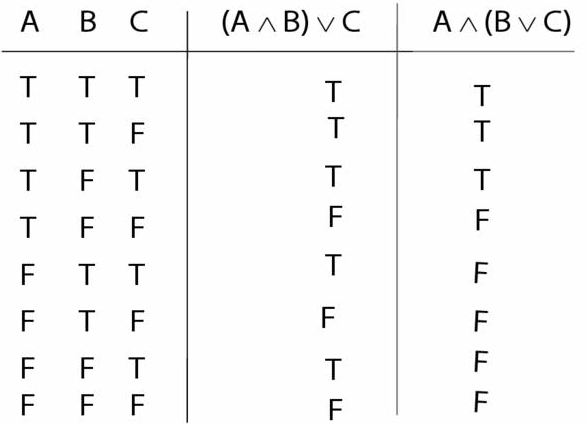
\includegraphics[scale=0.3]{img/tt_unit_153.png}
\end{center}
 
 
\section{A ∧ B ∨ C: They Are Different}
 
\begin{center}
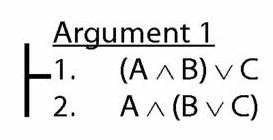
\includegraphics[scale=0.3]{img/arg1_unit_153.png}
\end{center}
\begin{center}
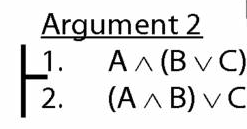
\includegraphics[scale=0.3]{img/arg2_unit_153.png}
\end{center}
\vfill

%--- end paste
%--------------- 
 


\end{multicols*}

\end{document}